\chapter{Appendices}\label{chapter:appendices}

\section{CAP Theorem}\label{section:appendices/CAP_theorem}
CAP Theorem was published by scientist Eric Brewer and also called as Brewer's Theorem. There are three major requirements for deploying an application in a distributed environment.
\begin{enumerate}
\item \textbf{Consistency}\\
A functionality of a service is accomplished as a whole or not at all. All the nodes accessing any data see the same version at any given time.
\item \textbf{Availability}\\
The functionalities provided by a service are available and working.
\item \textbf{Partition Tolerance}\\
The partitions which occurs due to problems in the network does not affect the operations of the system unless the whole network fails.
\end{enumerate}
According to the theorem, as the system scales across a number of nodes and the volume of requests increase, it becomes difficult to achieve all the three qualities but to compromise any one of them. \cite{Julian:2009aa}
Network partitions cannot be avoided completely due to the very nature of distributed system and so is the quality of partition tolerance has to be maintained. The choice is the trade off between availability and consistency. It is completely dependent upon business requirement which one to choose. \cite{Peter-Bailis:2013aa}
\section{Eventual Consistency}\label{section:appendices/eventual_consistency}
It is a weaker form of consistency which guarantees all read to a data item return the same value eventually, if no additional updates are performend to the same data item. For any update, only the nodes which are viable and reachable at the moment are updated and the remaining nodes are updated when they are back. \cite{Peter-Bailis:2013aa}
\section{Command Query Responsibility Segregation(CQRS)}\label{section:appendices/CQRS}
In this pattern as shown in the figure \ref{fig:appendices/cqrs}, the conceptual model is divided into two separate models, each one for update and read. It refers to creating different object model handled by different logical processes. The database can be shared, where it acts as integration point but can have different database as well.

\begin{figure}[H]
\begin{center}
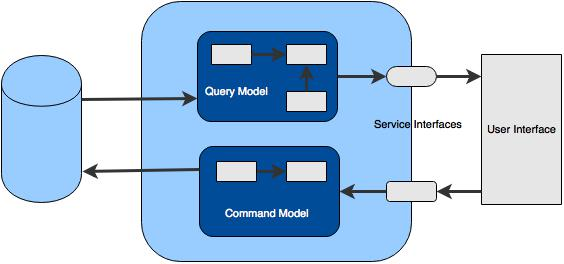
\includegraphics[width=0.8\textwidth]{figures/Appendices_one_cqrs}
\caption{CQRS [\cite{Fowler:2011ab}]}
\label{fig:appendices/cqrs}
\end{center}
\end{figure}